\section{Quick Sort}


\subsection{Definition}
\begin{itemize}
    \item basierend auf dem Divide-and-Conquer
    \item \textbf{Devide:} Auswahl eines zufälligen Elementes x (Pivot) und Aufteilung von S in:
    \begin{itemize}
        \item L Elemente kleiner als x
        \item E Elemente gleich x
        \item G Elemente grösser als x
    \end{itemize}
    \item \textbf{Recur:} sortiere L und G
    \item \textbf{Conquer:} vereine L, E and G
\end{itemize}
\vspace{-8pt}
\begin{center}
    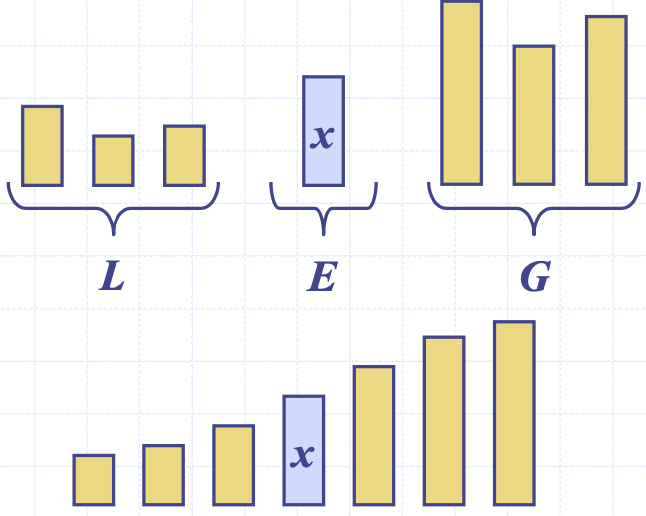
\includegraphics[scale=.3]{graphic/05 QuickSort/def.png}
\end{center}
\vspace{-8pt}


\subsection{Laufzeit}
\begin{itemize}
    \item Worst Case: $O(n^2)$ $\rightarrow$ Pivot Min- oder Max-Element
    \item Erwartet: O(n log (n))
    \begin{itemize}
        \item Good call: Länge von L und G sind beide kleiner als 3s/4
        \item Bad call: entweder L oder G ist länger als 3s/4 (s = länge)
        \item Aufruf ist ‘good’ mit einer Wahrscheinlichkeit von 1/2
    \end{itemize}
\end{itemize}
\begin{center}
    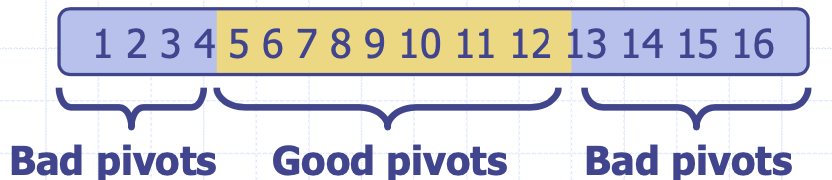
\includegraphics[scale=.3]{graphic/05 QuickSort/laufzeit.png}
\end{center}
\vspace{-8pt}


\subsection{Partitionierung}
\begin{itemize}
    \item Aufteilung der Input- Sequence:
    \begin{itemize}
        \item Entfernen von jeweils einem Element y von S
        \item einfügen von y in L, E oder G, abhängig vom Resultat des Vergleiches mit dem Pivot x
    \end{itemize}
    \item Aufteilung des Quick-Sort benötigt somit: O(n)
\end{itemize}


\subsection{Quick Sort Tree}
Ausführung eines Quick-Sort kann als binärer Baum dargestellt werden
\begin{itemize}
    \item Jeder Knoten repräsentiert einen rekursiven Aufruf des Quick- Sort und enthält:
    \begin{itemize}
        \item unsortierte Sequenz vor der Ausführung und sein Pivot
        \item sortierte Sequenz und sein Pivot nach dem Ende der Ausführung
    \end{itemize}
    \item Wurzel entspricht dem initialen Aufruf
    \item Blätter sind Aufrufe auf Teilsequenzen der Grösse 0 or 1
\end{itemize}
\vspace{-8pt}
\begin{center}
    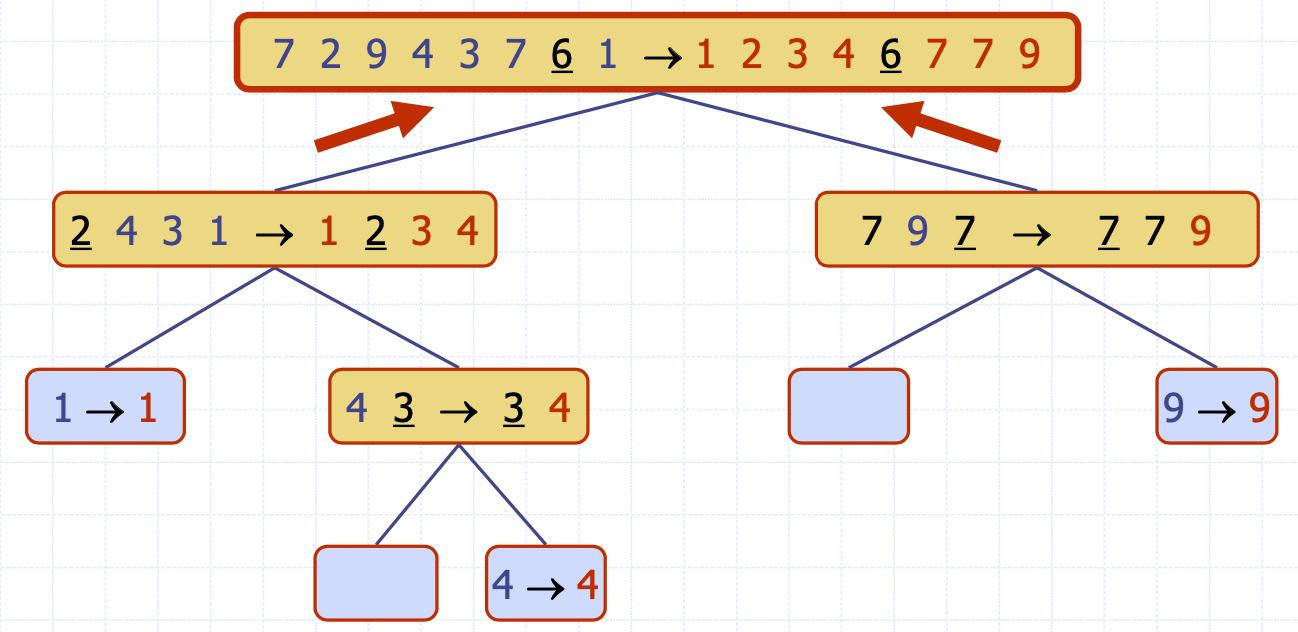
\includegraphics[scale=.2]{graphic/05 QuickSort/Quick Sort Tree.png}
\end{center}
\vspace{-8pt}


\subsection{In-Place Quick-Sort}
\begin{itemize}
    \item Quick-Sort kann ‘In-Place’ implementiert werden
    \item Partitionierungs-Schritt werden die Elemente der Input- Sequenz derart umgeordnet, dass:
    \begin{itemize}
        \item Elemente kleiner als das Pivot einen Index kleiner als h haben
        \item Elemente gleich dem Pivot einen Index zwischen h und k haben
        \item Elemente grösser als das Pivot einen Index grösser als k haben
    \end{itemize}
    \item rekursiven Calls betrachten
    \begin{itemize}
        \item Elemente mit Index kleiner als h
        \item Elemente mit Index grösser als k
    \end{itemize}
\end{itemize}
\subsubsection{Implementierung}
\begin{itemize}
    \item Partitionierung mit Benutzung zweier Indices um S in L und E \& G aufzuteilen.
\end{itemize}
\begin{center}
    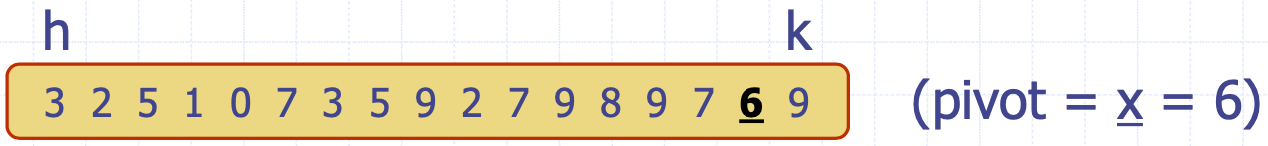
\includegraphics[scale=.2]{graphic/05 QuickSort/In-Place1.png}
\end{center}
\begin{itemize}
    \item Wiederholung bis h und k sich kreuzen:
    \begin{itemize}
        \item h nach rechts bis zu einem Element >= x
        \item k nach links bis zu einem Element < x
        \item Wenn h und k noch nicht gekreuzt: Elemente mit Indizes h und k vertauschen
    \end{itemize}
\end{itemize}
\vspace{-8pt}
\begin{center}
    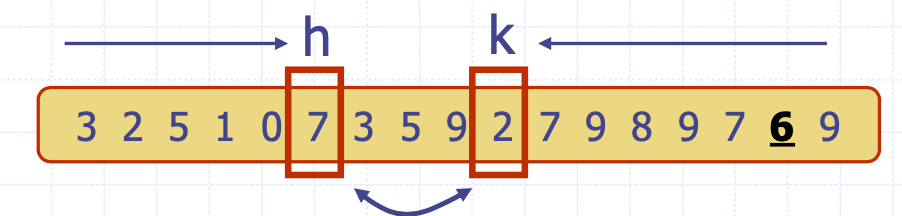
\includegraphics[scale=.2]{graphic/05 QuickSort/In-Place2.png}
\end{center}
\vspace{-8pt}
\begin{itemize}
    \item Pivot mit Element an Index h vertauschen
\end{itemize}


\section{Zusammenfassung Sortier-Algorithmen}
\begin{center}
    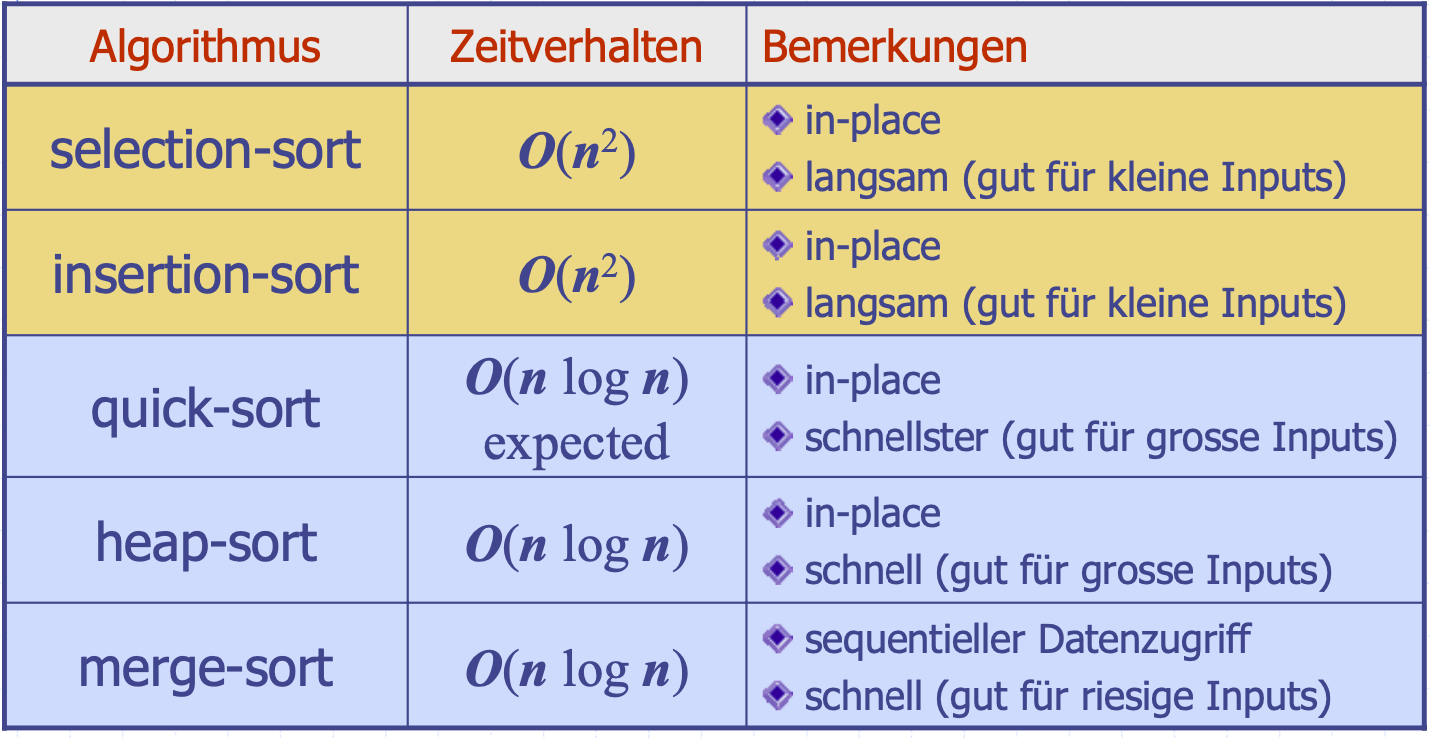
\includegraphics[scale=.25]{graphic/05 QuickSort/zfsg.png}
\end{center}
\vspace{-8pt}

\paragraph{In geordneter Reihenfolge}
h = $log_2$ $n$\\
$O(n$ $log_2 (n))$

\paragraph{als Pivot das letzte Element}
h = $n - 1$\\
$O(n^2)$\\
Besipiel mit n = 10:\\
$\sum_{i=1}^{n-1} i=\frac{(n-1) n}{2}=45 \text { Vergleiche total }$

\vfill
$ $
\columnbreak
